\documentclass[twoside,10pt]{article}
\usepackage{/Users/bradenhoagland/latex/styles/toggles}
%\toggletrue{sectionbreaks}
%\toggletrue{sectionheaders}
\newcommand{\docTitle}{Math 323 - HW 7}
\usepackage{/Users/bradenhoagland/latex/styles/common}
\importStyles{modern}{rainbow}{boxy}

%\renewcommand{\theenumi}{\alph{enumi}}

\begin{document}
%\tableofcontents

% ------------------------------
% 3.60
% ------------------------------
\begin{exer}[3.60]
	Describe how to trisect an obtuse angle with a compass and twice notched straightedge.
\end{exer}

Any obtuse angle can be decomposed into a right angle and an acute angle. We can easily trisect a right angle: Suppose $\angle CAB = 90\degree$ (as shown below), then form a circle $\mathcal{C}_{A}$ with radius less than $|AB|$. It intersects $AB$ at a point $D$. Now construct $\mathcal{C}_{D}(|AD|)$, and call the point of intersection of the two circles that lies inside of $\angle CAB$ the point $E$. Since $E$ is on both circles, and since both circles have the same radius, $|AE|=|ED|=|DE|$, i.e. $\Delta AED$ is an equilateral triangle. Thus $\angle EAD = 60\degree$, which means $\angle CAD = 30\degree = 90\degree /3$, so we have trisected $\angle CAB$.

\begin{figure}[H]
	\centering
	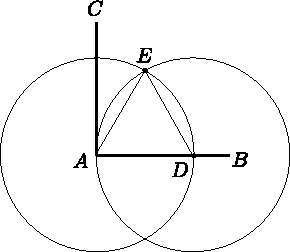
\includegraphics[scale=1]{fig/60.pdf}
	%\caption{}
\end{figure}

So given an obtuse angle, we first split it into a right angle and an acute angle. We trisect the right angle as above, then we trisect the acute angle as in the proof of Theorem 3.59. This gives us a trisection of the whole obtuse angle.

\newpage

% ------------------------------
% 5.3
% ------------------------------
\begin{exer}[5.3]
Show that each interior angle of a regular $n$-gon is $\frac{n-2}{n} \cdot 180\degree$.
\end{exer}

We will first show by induction that the interior angles of \textit{any} polygon (not necessarily regular) sum to $(n-2)\cdot 180\degree$. In the case of equilateral triangles ($n=3$), we know this to be true: the angles in a triangle must sum to $180\degree = (n-2) \cdot 180\degree$.

Now suppose the result holds for $n$-gons, then we want to show it also must hold for $(n+1)$-gons. Let $X_1\cdots X_{n+1}$ be a regular $(n+1)$-gon with points labeled clockwise, then we can decompose it into the $n$-gon $X_1\cdots X_{n}$ and the triangle $X_{n}X_{n+1}X_1$. By our inductive hypothesis and the fact that the interior angles of a triangles sum to $180\degree$, the sum of our $(n+1)$-gon's interior angles is
\[
        (n-2) \cdot 180\degree + 180\degree = \left( (n+1)-2 \right) \cdot 180\degree.
\] 

Now since we know we're working with \textit{regular} polygons, each of the interior angles must be the same. Thus each angle is
\[
\frac{n-2}{n} \cdot 180\degree.
\] 

\newpage

% ------------------------------
% 5.4
% ------------------------------
\begin{exer}[5.4]
Construct a regular triangle, square, pentagon, and hexagon, each with side length 2 inches.
\end{exer}

\begin{figure}[H]
	\centering
	\includegraphics[scale=0.05]{fig/4.pdf}
	%\caption{}
\end{figure}

% ------------------------------
% 5.5
% ------------------------------
\begin{exer}[5.5]
Construct models of the Platonic solids using the templates from the previous exercise.
\end{exer}

\begin{figure}[H]
	\centering
	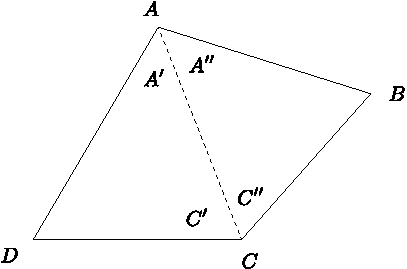
\includegraphics[scale=0.05]{fig/5.pdf}
	%\caption{}
\end{figure}

\newpage

We can answer the next three questions using the same method. Suppose we have a semiregular polyhedron represented by
\[
	(\underbrace{3, \dots, 3}_{m \text{ times}}, \underbrace{N, \dots, N}_{n \text{ times}}).
\] 
Let $F_{3}$ denote the number of triangular faces, and let $f_{N}$ denote the number of $n$-gonal faces. The number of vertices is
\[
	V = \frac{N F_{N}}{n} = \frac{3F_3}{m} ,
\] which implies $F_{3} = \frac{Nm}{3n} F_{N}$. Using this identity, the number of edges is
\[
E = \frac{3F_3+NF_{N}}{2} = \frac{Nm+Nn}{2n} F_{N}
\] and the number of faces is
\[
F = F_3 + F_N = \frac{3n+Nm}{3n} F_{N}.
\] Finally, we know that the Euler characteristic $\chi = V-E+F$ of this polyhedron is 2, so
\begin{align*}
	V-E+F &= \frac{N}{n}F_{N} - \frac{Nm+Nn}{2n} F_{N} + \frac{3n+Nm}{3n} F_{N} \\
	    2 &= \left( \frac{N(6-m-3n)+6n}{6n}  \right)F_{N} \\
	    F_{N} &= \frac{12n}{N(6-m-3n)+6n} .
\end{align*}

% ------------------------------
% 5.17
% ------------------------------
\begin{exer}[5.17]
How many pentagonal faces are on a snub dodecadehron?
\end{exer}

The snub dodecahedron has representation $(3,3,3,3,5)$, so $n=1,N=5$, and $m=4$. Thus $F_{5} = 12$.

% ------------------------------
% 5.18
% ------------------------------
\begin{exer}[5.18]
How many square faces are on a snub cube?
\end{exer}

The snub cube has representation $(3,3,3,3,4)$, so $n=1,N=4$, and $m=4$. Thus $F_{4}= 6$.

% ------------------------------
% 5.19
% ------------------------------
\begin{exer}[5.19]
	How many square faces are on a semiregular polyhedron represented by $(3,4,4,4)$?
\end{exer}

$n=3, N=4$, and $m=1$, so $F_{4}=18$.

\newpage

\end{document}
